\documentclass[tikz,convert=false]{standalone}
\usepackage{tikz}
\usetikzlibrary{arrows}

\begin{document}
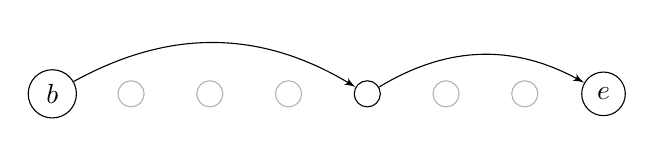
\begin{tikzpicture}
\tikzset{vertex/.style = {shape=circle,draw,minimum size=0.5em}}
\tikzset{edge/.style = {->,> = latex'}}

\node[vertex, draw=black   ] (a) at (0,0) {$b$};
\node[vertex, draw=black!30] (b) at (1,0) {};
\node[vertex, draw=black!30] (c) at (2,0) {};
\node[vertex, draw=black!30] (d) at (3,0) {};
\node[vertex, draw=black   ] (e) at (4,0) {};
\node[vertex, draw=black!30] (f) at (5,0) {};
\node[vertex, draw=black!30] (g) at (6,0) {};
\node[vertex, draw=black   ] (h) at (7,0) {$e$};

\draw[edge] (a) to[bend left] (e);
\draw[edge] (e) to[bend left] (h);
\end{tikzpicture}
\end{document}